\subsection{Testkonzept Software}\label{sec:testkonzeptSoftware}
Nach der Validierung der Hardware wird nun die Software getestet. Für einen einwandfreien Betrieb ist das Testen der Software einer der wichtigsten Bestandteile der Validierung. Gestartet wird mit der Validierung des PWM-Signals.

\subsubsection{PWM Signal}\label{sec: Validierung PWM Signal}

Das PWM Signal wurde ebenfalls mit einem 500Hz Sinus-Signal validiert. Dabei wurden die beiden PWM-Kanäle und das gefilterte Signal mit dem KO aufgezeichnet. Abbildung \ref{fig:Signal PWM Ausgänge} zeigt die gemessenen PWM-Kanäle.

\begin{figure}[H]
	\begin{center}
		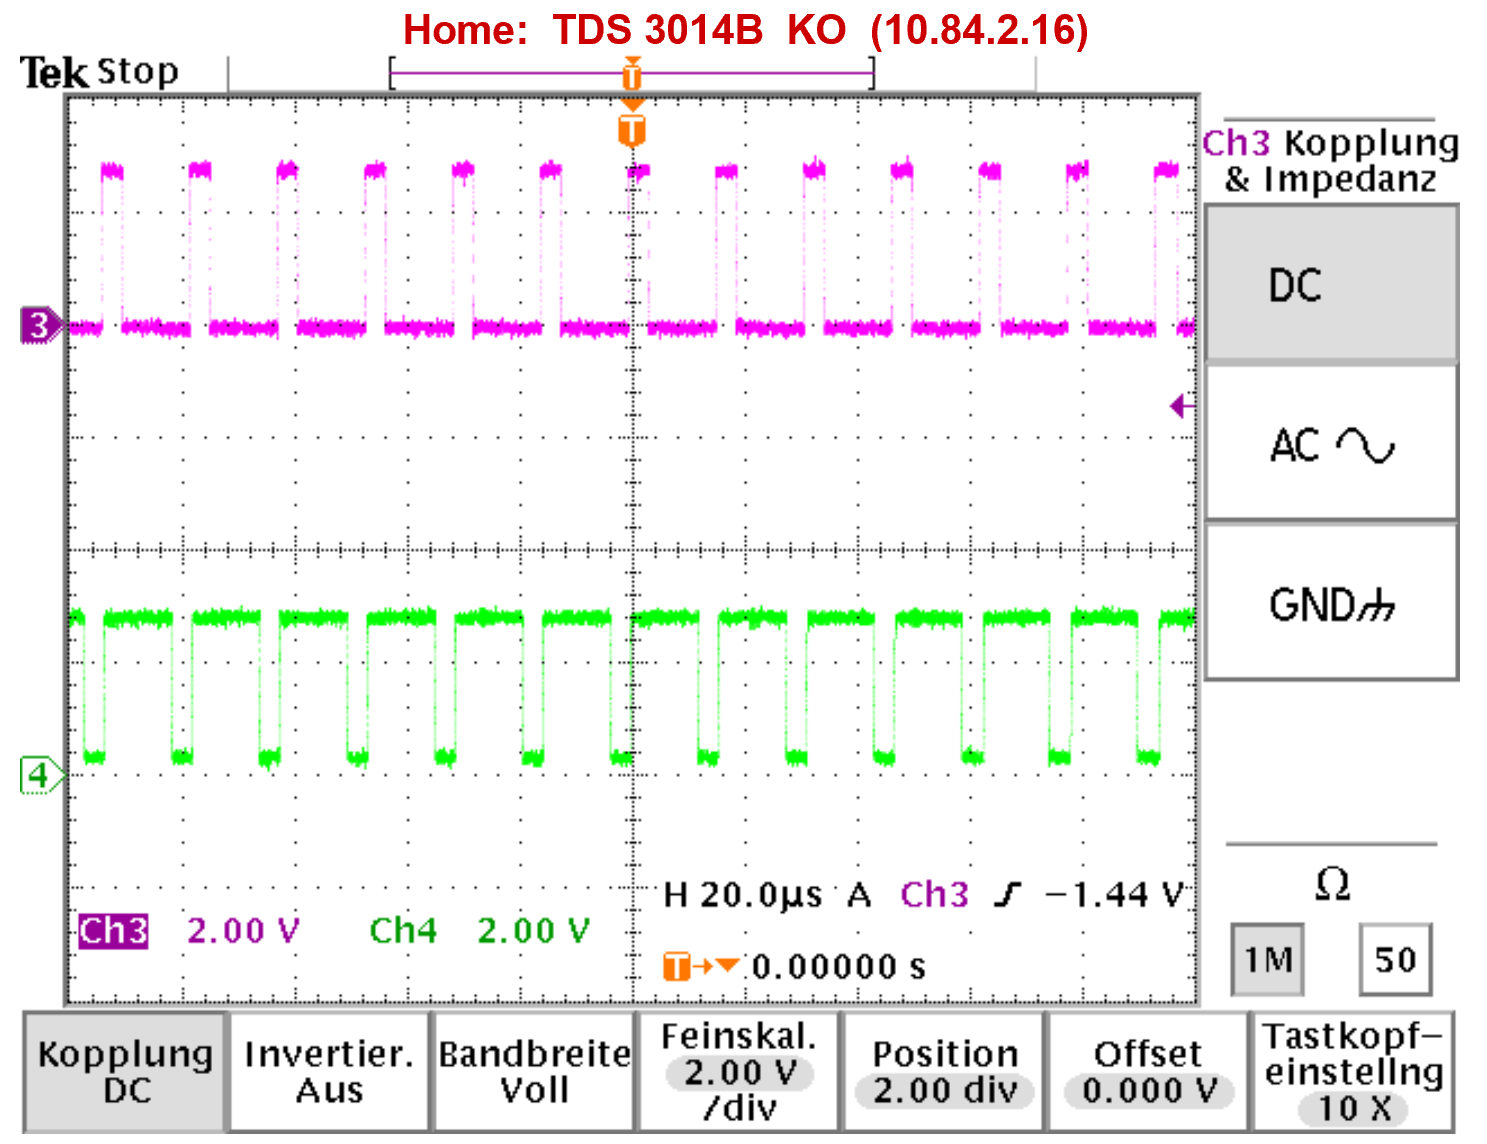
\includegraphics[width=120mm]{data/PWM_Signal_500Hz_Mono_mit_Infos.png}
		\caption[PWM Signal beider PWM Ausgänge]{PWM Signal beider PWM Ausgänge} %picture caption
		\label{fig:Signal PWM Ausgänge}
	\end{center}
\end{figure}


Aus der Abbildung \ref{fig:Signal PWM Ausgänge} ist ersichtlich, dass die beiden PWM-Signale zwar invertiert zu einander stehen, aber auch zeitlich (knapp $4\mu s$) verschoben sind. Diese Zeitverschiebung hat jedoch keinen hörbaren Effekt und kann somit vernachlässigt werden. Um die Einstellungen des PWM-Moduls aus \ref{sec:audioPWM} zu validieren, wurde ein $500Hz$ Sinus-Signal mit dem KO abgebildet. Das entstandene Resultat ist in nachfolgender Abbildung \ref{fig:PWM Topval 500 Stereo} links ersichtlich. Dabei beträgt die Frequenz des Signals nur $127Hz$ anstatt den angelegten $500Hz$. Das entspricht einem Faktor von rund $4$. Um die gewünschten $500Hz$ zu erreichen, wurde der top value aus Kapitel \ref{sec:PWM initialisieren} von $500$ auf $125$ herunter gesetzt. Das entstandene Resultat ist in Abbildung \ref{fig:PWM Topval 500 Stereo} rechts ersichtlich. Das Sinus-Signal schwingt nun mit $500Hz$. Da die Berechnungen einen top value von $500$ ergeben, deutet dies auf einen Fehler im Code, in der Audiodatei oder auf einen Überlegungsfehler hin. Es wurde festgestellt, dass die Tests fälschlicherweise mit einer Audiodatei vom Typ Stereo durchgeführt wurden. Da jedoch nur ein Kanal angesteuert wird, ergibt sich daraus ein Unterschied mit dem Faktor $2$ zu den Berechnungen. Dieser Test wurde folglich noch einmal mit einer Mono-Audiodatei durchgeführt, wobei sich der top value gemäss den Erwartungen um den Faktor $2$ vom berechneten Wert unterscheidet.

\begin{figure}[htbp]
	\centering
	\subfigure[PWM auf $32kHz$ eingestellt]{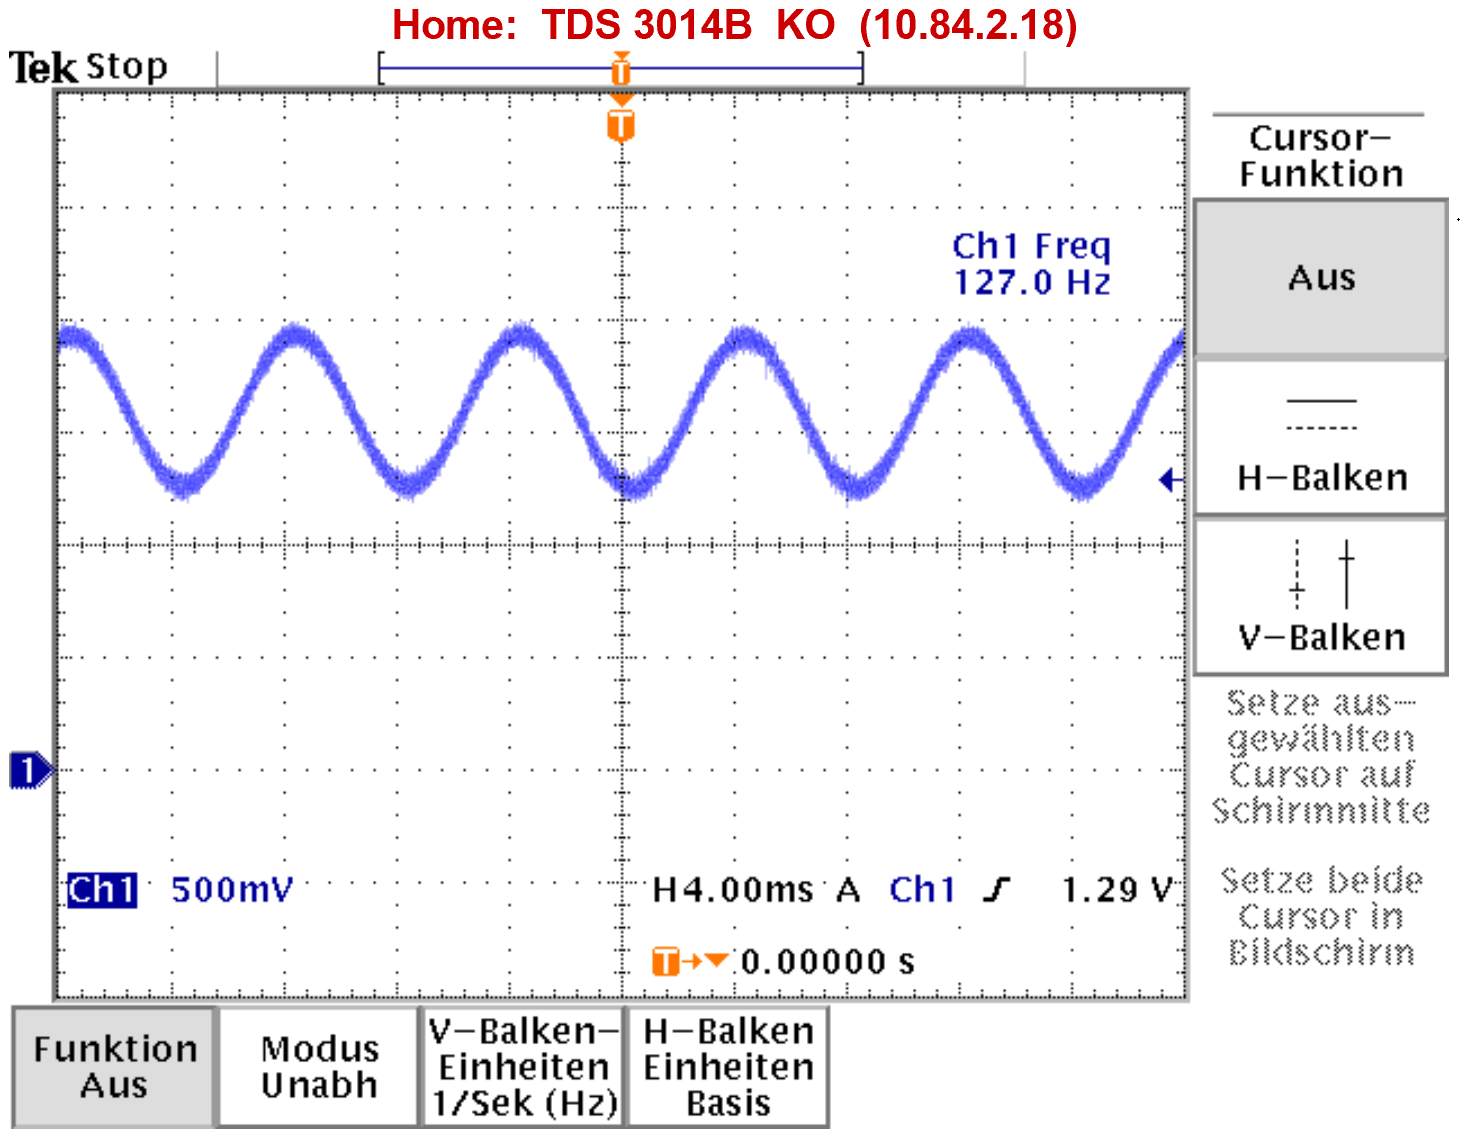
\includegraphics[width = 0.48\textwidth]{data/TOPVAL_Stereo_500.png}}\quad
	\subfigure[PWM auf $128kHz$ eingestellt]{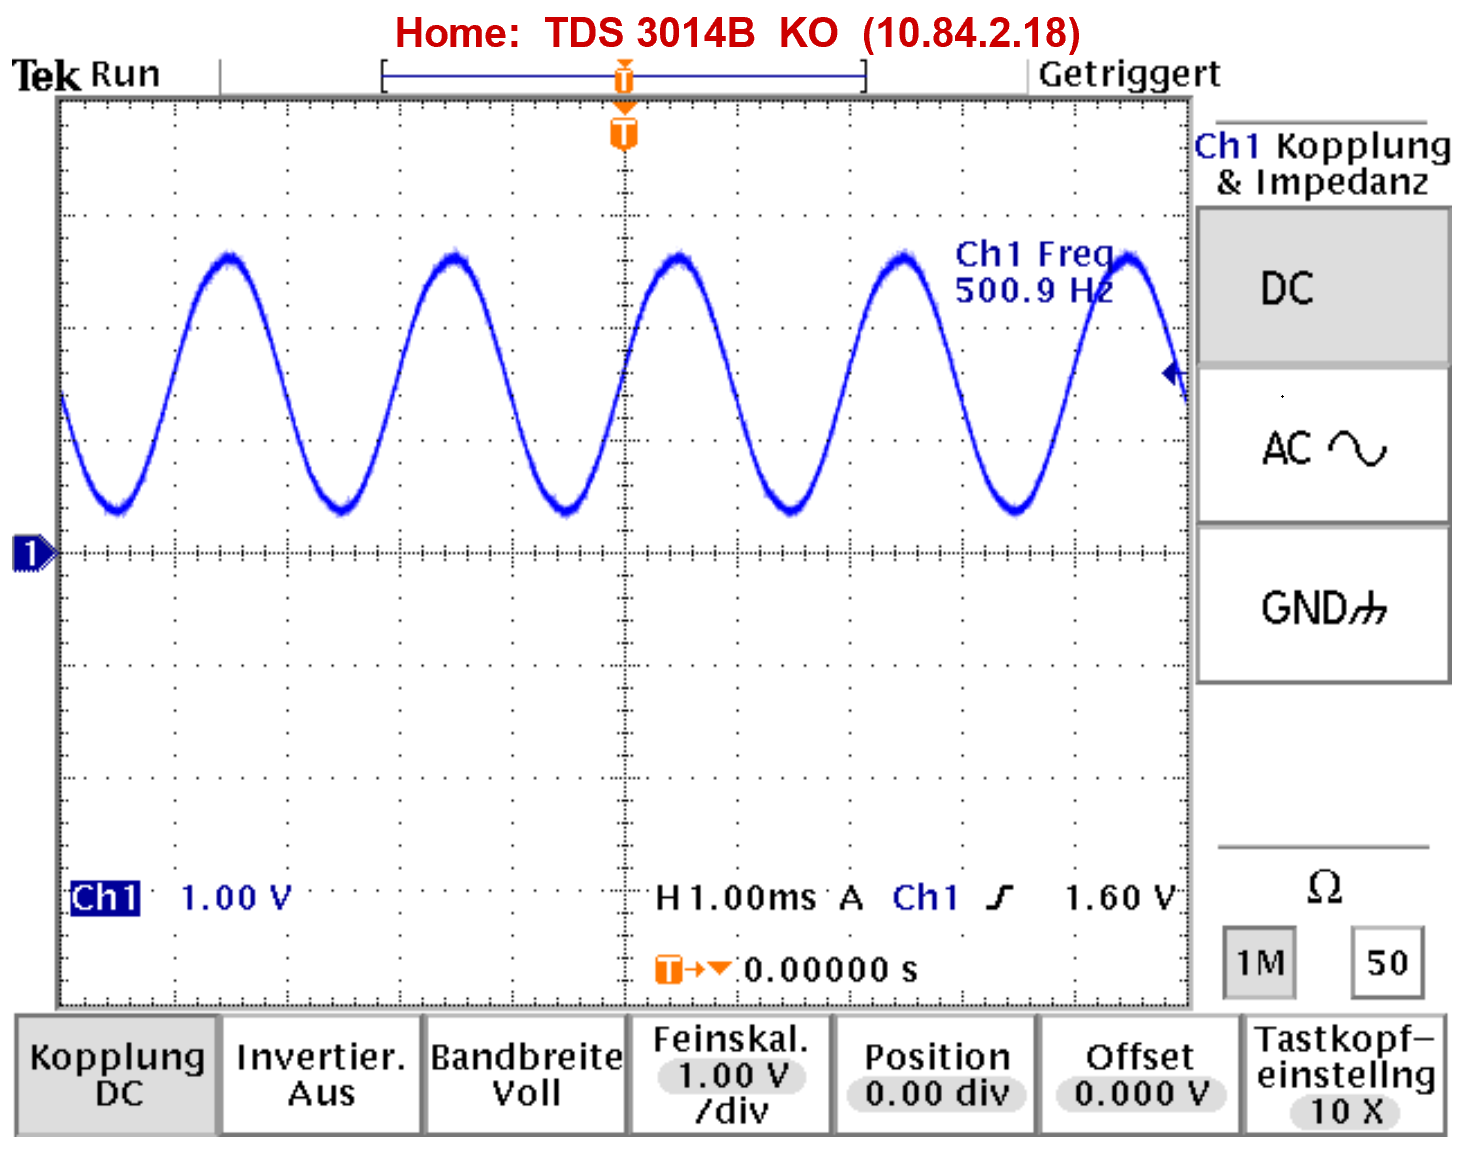
\includegraphics[width = 0.48\textwidth]{data/TOPVAL_Stereo_125.png}}\quad
	\caption[PWM auf $128kHz$ eingestellt]{Aufnahme der Filterstufe: links ohne Filterstufe und rechts mit Filterstufe}
	\label{fig:PWM Topval 500 Stereo}
\end{figure}

\subsubsection{Statemachine}
Die Statemachine wurde auf ihr Verhalten hin getestet. Dabei wurden alle States mithilfe von Flags einmal erzwungen, wobei folgende States nicht korrekt funktionierten:

\begin{itemize}
	\item ADC-Batterie 
	\item Shutdown
	\item Merken Liste Löschen
	\item Charge
\end{itemize}

Dabei ist es wichtig zu erwähnen, dass diese {\glqq fehlerhaften States\grqq} in der Statemachine eigentlich funktionieren, jedoch ihre Aufgabe nicht erfüllen können, da sie aus zeitlichen Gründen nicht implementiert wurden. Die Implementierung dieser States kann bei der Weiterverfolgung dieses Projektes als zusätzlicher Arbeitsschritt implementiert werden.

\subsubsection{Bluetooth}
Das Bluetooth Modul wurde mit verschiedenen Beacons getestet. Dabei is aufgefallen, dass bei der gleichzeitigen Verwendung von mehreren Beacons, welche mit unterschiedlichen Sendeintervallen senden, es zu grösseren Problemen führt. Es dominieren die Beacons mit schnellerer Sendefrequenz, wobei die langsameren überdeckt werden. Aus diesem Grund ist es zu empfehlen, dass die Abstände der Beacons gemäss Abbildung \ref{fig:ref_felder} verwendet werden. Die Radien können für jeden Beacon einzeln konfiguriert werden. Die Grösse des Radius kann zwischen $0m$ und $40m$ variieren. Als Standardwert ist dieser Radius auf $3m$ eingestellt.

\begin{figure}[H]
	\begin{center}
		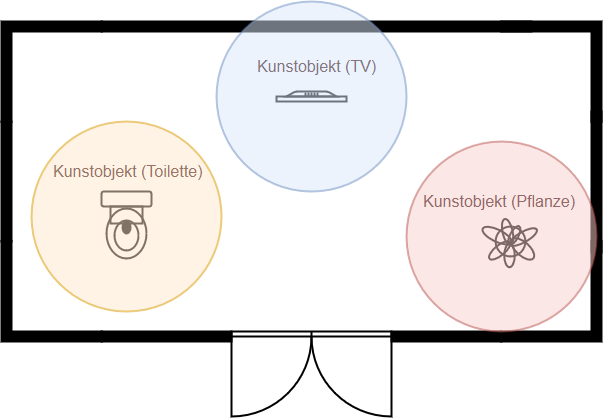
\includegraphics[width=120mm]{data/validierung_software_ref_felder.png}
		\caption[Überlappung der Referenz-Felder]{Überlappung der Referenz-Felder} %picture caption
		\label{fig:ref_felder}
	\end{center}
\end{figure}

\subsubsection{SD-Karte}
Das SD-Karten Modul hat alle Anforderungen erfüllt. Das Lesen und Schreiben ist problemlos möglich und funktioniert einwandfrei. Einziger Fehler ist in der Funktion \glqq Merken\grqq (welche vom \glqq Like Button\grqq aufgerufen wird) zu verzeichnen. Hierbei ist es nicht möglich, ein gemerktes Kunstobjekt wieder zu löschen. Dafür ist es notwendig die SD-Karte aus dem Gerät zu entnehmen und sie neu zu konfigurieren. Zudem kann man ein Kunstobjekt gleich mehrmals in die gleiche {\glqq Merkliste\grqq} einfügen, was zwar keine Probleme im Gerät auslöst, sich aber als relativ unpraktisch erweist.


